\chapter{Studi Literatur}

\section{Qubit}
\par
Dalam sistem komputasi klasik, bit merupakan satuan informasi paling dasar yang hanya dapat memiliki dua keadaan diskrit, yaitu 0 atau 1 \cite{nielsen2010quantum}. Setiap operasi logika dalam komputer klasik dibangun dari manipulasi terhadap bit-bit ini, yang secara fisik dapat direpresentasikan oleh dua kondisi berbeda, seperti arus listrik yang mengalir atau tidak mengalir, tegangan tinggi atau rendah, serta keadaan magnetik utara atau selatan \cite{tanenbaum2013structured}. Dengan demikian, bit berfungsi sebagai pembawa informasi biner yang menjadi fondasi bagi seluruh proses komputasi konvensional \cite{shannon1948mathematical}.
\par
Namun, seiring berkembangnya pemahaman terhadap prinsip-prinsip mekanika kuantum, muncul paradigma baru dalam penyimpanan dan pemrosesan informasi yang dikenal sebagai qubit (quantum bit) \cite{nielsen2010quantum}. Tidak seperti bit klasik yang hanya dapat berada dalam satu keadaan tertentu pada satu waktu, qubit mampu berada dalam superposisi antara keadaan $\ket{0}$ dan $\ket{1}$ secara bersamaan \cite{dirac1981principles}. Transisi dari bit ke qubit ini menandai pergeseran fundamental dari logika deterministik menuju logika probabilistik-kuantum, di mana informasi tidak lagi direpresentasikan secara biner murni, melainkan sebagai vektor dalam ruang Hilbert dua dimensi yang memiliki representasi matriks sebagai berikut \cite{sakurai2017modern}.

\begin{equation}
    \ket{0} = \begin{pmatrix} 1 \\ 0 \end{pmatrix}
\end{equation}
dan
\begin{equation}
    \ket{1} = \begin{pmatrix} 0 \\ 1 \end{pmatrix}
\end{equation}
\par
Kombinasi linier dari dua qubit atau basis vektor yang menyatakan keadaan informasi kuantum secara umum dituliskan menjadi
\begin{equation}
\ket{\psi} = \alpha \ket{0} + \beta \ket{1}\label{keadaanumum}
\end{equation}
dengan $\alpha$ dan $\beta$ adalah bilangan kompleks. Keadaan tersebut harus memenuhi syarat normalisasi atau $\langle \psi | \psi \rangle = 1$. Sehingga $\alpha$ dan $\beta$ harus memenuhi
\begin{equation}
|\alpha|^2 + |\beta|^2 = 1
\end{equation}

\par
Sistem yang terdiri atas lebih dari satu qubit maka keadaan sistemnya dapat dinyatakan dengan perkalian langsung dari masing-masing keadaannya \cite{mermin2007quantum, bengtsson2017geometry, barnett2009quantum, schlosshauer2007decoherence}. Misalkan informasi yang dimiliki yaitu bilangan 2 dan 6 yang apabila dinyatakan dalam bit klasik akan menjadi 10 dan 110. Informasi tersebut jika dinyatakan secara kuantum maka dapat dituliskan menjadi
\begin{equation}
10 \rightarrow \ket{1} \otimes \ket{0}
\end{equation}
dan
\begin{equation}
110 \rightarrow \ket{1} \otimes \ket{1} \otimes \ket{0}
\end{equation}
atau secara ringkas juga dapat dituliskan menjadi
\begin{equation}
\ket{1} \otimes \ket{0} = \ket{10}
\end{equation}
dan
\begin{equation}
\ket{1} \otimes \ket{1} \otimes \ket{0} = \ket{110}
\end{equation}
\par

Qubit juga memiliki realitas fisis, beberapa diantaranya adalah pada kasus polarisasi foton \cite{nielsen2010quantum}. Pada polarisasi, $\ket{0}$ merupakan representasi dari polarisasi vertikal foton, sedangkan $\ket{1}$ untuk polarisasi horizontalnya \cite{kok2007linear}. Qubit juga dapat digunakan menjadi representasi dari spin elektron, misalnya $\ket{0}$ adalah representasi dari spin-up dan $\ket{1}$ sebagai spin-down \cite{sakurai2017modern}.

\subsection{Representasi Bola Bloch}
\par
Suatu keadaan qubit dapat direpresentasikan dalam bola Bloch. Dengan mengambil bentuk polar pada koefisien dalam persamaan (\ref{keadaanumum}), yaitu $\alpha = |\alpha| e^{i\varphi_\alpha}$ dan $\beta = |\beta| e^{i\varphi_\beta}$, maka persamaan (\ref{keadaanumum}) dapat dituliskan sebagai
\begin{equation}\label{kk}
	\ket{\psi}=|\alpha| e^{i\varphi_\alpha}\ket{0}+|\beta| e^{i\varphi_\beta}\ket{1}.
\end{equation}
Karena $|\alpha|^2 + |\beta|^2 = 1$, maka koefisien tersebut dapat diparameterisasi sebagai
\begin{equation}
	|\alpha|=\cos \theta, \ |\beta|=\sin \theta,
\end{equation}
dengan $\cos\theta$ dan $\sin\theta$ bernilai positif sehingga parameter $\theta$ dibatasi pada rentang $0 \leq \theta \leq \frac{\pi}{2}$ \cite{Blumel}.
\par
Selanjutnya, persamaan (\ref{kk}) dapat dituliskan sebagai
\begin{equation}
	\begin{aligned}
		\ket{\psi} &= \cos \theta \, e^{i\varphi_\alpha} \ket{0} + \sin \theta \, e^{i\varphi_\beta} \ket{1} \\
		&= e^{i\varphi_\alpha} \left( \cos \theta \ket{0} + \sin \theta \, e^{i(\varphi_\beta - \varphi_\alpha)} \ket{1} \right).
	\end{aligned}
\end{equation}
Faktor global $e^{i\varphi_\alpha}$ dapat diabaikan karena tidak bersifat observabel. Dengan mendefinisikan $\varphi = \varphi_\beta - \varphi_\alpha$, persamaan di atas menjadi
\begin{equation}\label{poin}
	\ket{\psi} = \cos\theta \ket{0} + \sin\theta \, e^{i\varphi} \ket{1}.
\end{equation}
\par
Jika dilakukan substitusi $\theta \Rightarrow \frac{\theta}{2}$, maka persamaan di atas dapat dituliskan sebagai
\begin{equation}\label{bloch}
	\ket{\psi} = \cos \frac{\theta}{2} \ket{0} + \sin \frac{\theta}{2} \, e^{i\varphi} \ket{1}.
\end{equation}

Persamaan tersebut merepresentasikan keadaan qubit dalam bola Bloch, seperti ditunjukkan pada Gambar~(\ref{fig:Blochsphere}), dengan batasan $0 \leq \theta \leq \pi$ dan $0 \leq \varphi \leq 2\pi$.
\begin{figure}[htbp]
	\centering
	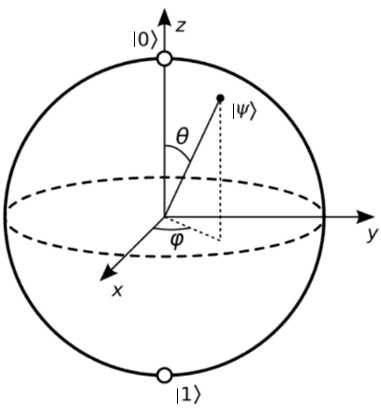
\includegraphics[width=0.6\textwidth]{Bloch_Sphere} % sesuaikan path dan ukuran gambar
	\caption{Bola Bloch}
	\label{fig:Blochsphere}
	\cite{Meoijuan}
\end{figure}

Keadaan qubit dapat direpresentasikan sebagai titik-titik pada permukaan bola Bloch. Titik-titik tersebut dapat dinyatakan dalam koordinat Kartesian ($x$, $y$, $z$), dengan
\begin{equation}
	\begin{aligned}
		x &= \sin\theta \cos\varphi, \\
		y &= \sin\theta \sin\varphi, \\
		z &= \cos\theta.
	\end{aligned}
\end{equation}
Dengan demikian, vektor pada bola Bloch dapat dituliskan sebagai \cite{pathak2013elements}
\begin{equation}\label{nn}
	\begin{aligned}
		\hat{n} &= x \, \hat{i} + y \, \hat{j} + z \, \hat{k} \\
		&= \sin\theta \cos\varphi \, \hat{i} + \sin\theta \sin\varphi \, \hat{j} + \cos\theta \, \hat{k}.
	\end{aligned}
\end{equation}

\subsection{Keadaan Dua Qubit}
Keadaan umum untuk dua qubit adalah
\begin{equation}
	\ket{\psi}=c_{00}\ket{00}+c_{01}\ket{01}+c_{10}\ket{10}+c_{11}\ket{11}
\end{equation}
dengan koefisien kompleks yang memenuhi
\begin{equation}
    |c_{00}|^2+|c_{01}|^2+|c_{10}|^2+|c_{11}|^2=1
\end{equation}
\par
Persamaan umum untuk keadaan qubit rangkap dua tersebut jika disederhanakan dalam bentuk notasi sigma adalah sebagai berikut
\begin{equation}
    \ket{\psi}=\sum_{i_1,i_2=0}^{1} c_{i_1 i_2} \ket{i_1 i_2}\label{umum2qubit}
\end{equation}
Contoh keadaan untuk dua qubit adalah
\begin{equation}
	\ket{\psi_1}=\frac{1}{2}(\ket{00}+\ket{01}+\ket{10}+\ket{11})
\end{equation}
dengan $c_{00}=c_{01}=c_{10}=c_{11}=\frac{1}{2}$,
\begin{equation}
	\ket{\psi_2}=\frac{1}{2}(\ket{00}+\ket{01}+\ket{10}-\ket{11})
\end{equation}
dengan $c_{00}=c_{01}=c_{10}=-c_{11}=\frac{1}{2}$,
\begin{equation}
	\ket{\psi_3}=\frac{1}{2}(\ket{00}+\ket{01}-\ket{10}-\ket{11})
\end{equation}
dengan $c_{00}=c_{01}=-c_{10}=-c_{11}=\frac{1}{2}$,
\begin{equation}
	\ket{\psi_4}=0,1\ket{00}+0,5\ket{01}+0,5\ket{10}+0,7\ket{11}
\end{equation}
dengan $c_{00}=0,1, c_{01}=c_{10}=0,5, c_{11}=0,7$, dan
\begin{equation}
	\ket{\psi_5}=\frac{1}{\sqrt{2}}(\ket{00}+\ket{11})
\end{equation}
dengan $c_{00}=c_{11}=\frac{1}{\sqrt{2}}$ dan $c_{01}=c_{10}=0$.

\subsection{Keadaan Tiga Qubit}
Keadaan umum untuk tiga qubit adalah
\begin{equation}
	\ket{\psi}=c_{000}\ket{000}+c_{001}\ket{001}+c_{010}\ket{010}+c_{011}\ket{011}+c_{100}\ket{100}+c_{101}\ket{101}+c_{110}\ket{110}+c_{111}\ket{111}
\end{equation}
dengan koefisien kompleks yang memenuhi
\begin{equation}
	|c_{000}|^2+|c_{001}|^2+...+|c_{111}|^2=1
\end{equation}
\par
Persamaan umum untuk keadaan qubit rangkap tiga tersebut jika disederhanakan dalam bentuk notasi sigma adalah sebagai berikut
\begin{equation}
	\ket{\psi}=\sum_{i_1,i_2,i_3=0}^{1} c_{i_1 i_2,i_3} \ket{i_1 i_2 i_3 }\label{umum3qubit}
\end{equation}
Contoh keadaan untuk dua qubit adalah
\begin{equation}
	\ket{\psi_1}=\frac{1}{2\sqrt{2}}(\ket{000}+\ket{001}+\ket{010}+\ket{011}+\ket{100}+\ket{101}+\ket{110}+\ket{111})
\end{equation}
dengan $c_{000}=c_{001}=...=c_{111}=\frac{1}{2\sqrt{2}}$,
\begin{equation}
	\ket{\psi_2}=\frac{1}{\sqrt{2}}(\ket{000}+\ket{111})
\end{equation}
dengan $c_{000}=c_{111}=\frac{1}{\sqrt{2}}$ dan $c_{001}=c_{010}=c_{110}=0$, dan
\begin{equation}
	\ket{\psi_3}=\frac{1}{\sqrt{3}}(\ket{001}+\ket{010}+\ket{100})
\end{equation}
dengan $c_{001}=c_{010}=c_{100}=\frac{1}{\sqrt{3}}$ dan koefisien yang lainnya bernilai 0.

\subsection{Keadaan n-Qubit}
\par
Sistem kuantum yang terdiri atas lebih dari satu qubit merupakan fondasi utama dalam teori informasi kuantum, komputasi kuantum, serta kajian keterikatan kuantum multipartit. Secara matematis, keadaan sistem kuantum multipartit direpresentasikan dalam ruang Hilbert hasil kali tensor dari ruang Hilbert masing-masing subsistem \cite{nielsen2010quantum}. Generalisasi konsep ini pada sistem dengan $n$ qubit menghasilkan struktur ruang keadaan yang jauh lebih kompleks, dengan dimensi ruang Hilbert sebesar $2^n$ \cite{preskill_lecture_notes}. Secara umum kombinasi linier untuk sistem dengan keadaan n qubit dapat dituliskan sebagai berikut
\begin{equation}
	\ket{\psi}=c_{00...0}\ket{00...0}+c_{00...10}\ket{00...10}+...+c_{11...1}\ket{11...1}
\end{equation}
atau
\begin{equation}
	\ket{\psi}=\sum_{i_1,i_2,...,i_n}^1 c_{i_1 i_2...i_n}\ket{i_1 i_2...i_n}
\end{equation}
dengan
\begin{equation}
	\sum_{i_1,i_2,...,i_n=0}^{1}|c_{i_1 i_2...i_n}|^2=1
\end{equation}

Keadaan n-qubit yang dapat dituliskan sebagai hasil kali tensor dari keadaan masing-masing qubit disebut sebagai keadaan terpisah (separable state). Sebaliknya, apabila keadaan tersebut tidak dapat direpresentasikan dalam bentuk hasil kali tensor sederhana, maka keadaan tersebut tergolong sebagai keadaan terikat (entangled state) \cite{horodecki2009quantum}. Fenomena keterikatan kuantum ini menjadi ciri khas utama mekanika kuantum dan memainkan peran penting dalam berbagai aplikasi kuantum modern, termasuk teleportasi kuantum, kriptografi kuantum, dan komputasi kuantum \cite{bennett_1993}.

\section{Keterbelitan}
\par
Suatu keadaan murni $\ket{\psi_{12}}$ dikatakan terbelit jika dan hanya jika tidak memenuhi
\begin{equation}
	\ket{\psi_{12}}=\ket{\psi_1}\otimes\ket{\psi_2}
\end{equation}
atau dikatakan sebagai keadaan tidak terpisah (\textit{non-separable}). Jika memenuhi maka dikatakan keadaan terpisah (\textit{separable}) \cite{esteve2004quantum}.
\par
Untuk memahami pernyataan di atas, dimisalkan $\ket{\psi_1}$ dan $\ket{\psi_2}$ dalam keadaan dua qubit sebagai berikut
\begin{equation}
		\ket{\psi_1}=x_0\ket{0}+x_1\ket{1}\\
		\ket{\psi_2}=y_0\ket{0}+y_1\ket{1}
\end{equation}
dan suatu keadaan dua qubit yang belum diketahui keterbelitannya
\begin{equation}
		\ket{\psi_{12}}=c_{00}\ket{00}+c_{01}\ket{01}+c_{10}\ket{10}+c_{11}\ket{11}
\end{equation}
di mana
\begin{align}
    c_{00}=x_0y_0
    \label{eq:terbelit1}\\
    c_{01}=x_0y_1
    \label{eq:terbelit2}\\
    c_{10}=x_1y_0
    \label{eq:terbelit3}\\
    c_{11}=x_1y_1
    \label{eq:terbelit4}
\end{align}
Jika koefisien $c_{00}$, $c_{01}$, $c_{10}$, dan $c_{11}$ berturut-turut bisa diuraikan dalam perkalian $x_0y_0$, $x_0y_1$, $x_1y_0$, dan $x_1y_1$, maka keadaan dikatakan terpisah. Jika tidak bisa diuraikan dalam perkalian tersebut, maka keadaan dikatan terbelit \cite{taufiqi2024asymmetric}.
\subsection{Keterbelitan Keadaan Dua Qubit}
Kembali pada persamaan keadaan dua qubit (\ref{umum2qubit}), yaitu $\ket{\psi}=\sum_{i_1,i_2=0}^{1} c_{i_1 i_2} \ket{i_1 i_2}$
\subsubsection{Keadaan Terpisah}
Misalkan ada dua keadaan qubit tunggal
\begin{equation}
	\ket{\psi_1}=x_0\ket{0}+x_1\ket{1},
\end{equation}
\begin{equation}
	\ket{\psi_2}=y_0\ket{0}+y_1\ket{1}
\end{equation}
dan
\begin{align}
	\ket{\psi}=\ket{\psi_1}\otimes\ket{\psi_2}\\
	&=(x_0\ket{0}+x_1\ket{1})\otimes(y_0\ket{0}+y_1\ket{1})\\
	&=x_0y_0\ket{00}+x_0y_1\ket{01}+x_1y_0\ket{10}+x_1y_1\ket{11}
\end{align}

Koefisien untuk keadaan terpisah yang telah dipaparkan pada persamaan (\ref{eq:terbelit1}), (\ref{eq:terbelit2}), (\ref{eq:terbelit3}), dan (\ref{eq:terbelit4}) dapat dituliskan sebagai berikut.
\begin{align}
	c_{00} &= x_0 y_0 \nonumber \\
	c_{01} &= x_0 y_1 \nonumber \\
	c_{10} &= x_1 y_0 \nonumber \\
	c_{11} &= x_1 y_1 \label{koefisien2qubit}.
\end{align}
Ditinjau contoh keadaan dua qubit $|\phi_1\rangle$ sebagai berikut

\begin{equation}
|\phi_1\rangle =
\frac{1}{2}
\left(
|00\rangle - |01\rangle + |10\rangle - |11\rangle
\right).
\end{equation}
dengan $c_{00}=-c_{01}=c_{10}=-c_{11}=\frac{1}{2}$

Untuk mencari nilai dari masing-masing koefisien, kita bisa melakukan perhitungan berikut.

\begin{equation}
\frac{c_{00}}{c_{01}}=\frac{x_0y_0}{x_0y_1} = \frac{y_0}{y_1}=\frac{1/2}{-1/2}=-1
\end{equation}
sehingga $y_0=-y_1=\frac{1}{\sqrt{2}}$ dan

\begin{equation}
	\frac{c_{00}}{c_{10}}=\frac{x_0y_0}{x_1y_0} = \frac{x_0}{x_1}=\frac{1/2}{1/2}=1
\end{equation}
sehingga $x_0=x_1=\frac{1}{\sqrt{2}}$.
Sedangkan
\begin{equation}
	\frac{c_{11}}{c_{01}}=\frac{x_1y_1}{x_0y_1} = \frac{x_1}{x_0}=\frac{-1/2}{-1/2}=1
\end{equation}
sehingga $x_0=x_1=\frac{1}{\sqrt{2}}$ dan
\begin{equation}
	\frac{c_{11}}{c_{10}}=\frac{x_1y_1}{x_1y_0} = \frac{y_1}{y_0}=\frac{-1/2}{1/2}=-1
\end{equation}
sehingga $y_1=-y_0=\frac{1}{\sqrt{2}}$
maka
\begin{equation}
	\ket{\psi_1}=\frac{1}{\sqrt{2}}(\ket{0+\ket{1}})
\end{equation}
\begin{equation}
	\ket{\psi_2}=\frac{1}{\sqrt{2}}(\ket{0-\ket{1}})
\end{equation}

Karena hasil pada persamaan $x_0$ dan $x_1$ serta $y_0$ dan $y_1$konsisten menggunakan cara apapun, maka keadaan $|\phi_1\rangle$ memiliki solusi yang pasti untuk nilai koefisien $x_0, x_1, y_0,$ dan $y_1$,
sehingga keadaan $|\phi_1\rangle$ adalah keadaan yang terpisah.

\begin{equation}
|\phi_1\rangle =
\frac{1}{\sqrt{2}}
\left(
|0\rangle + |1\rangle
\right)
\otimes
\frac{1}{\sqrt{2}}
\left(
|0\rangle - |1\rangle
\right).
\end{equation}

\subsubsection{Keadaan Terbelit}
Ditinjau contoh keadaan yang lain $|\phi_2\rangle$ sebagai berikut

\begin{equation}\label{phi2}
|\phi_2\rangle =
\frac{1}{2}
\left(
|00\rangle + |01\rangle + |10\rangle - |11\rangle
\right).
\end{equation}
dengan $c_{00}=c_{01}=c_{10}=-c_{11}=\frac{1}{2}$

Untuk mencari nilai dari masing-masing koefisien, kita bisa melakukan perhitungan berikut.
\begin{equation}
	\frac{c_{00}}{c_{10}}=\frac{x_0y_0}{x_1y_0} = \frac{x_0}{x_1}=\frac{1/2}{1/2}=1
\end{equation}
sehingga $x_0=x_1=\frac{1}{\sqrt{2}}$.
Sedangkan
\begin{equation}
	\frac{c_{11}}{c_{01}}=\frac{x_1y_1}{x_0y_1} = \frac{x_1}{x_0}=\frac{-1/2}{1/2}=-1
\end{equation}
sehingga $x_0=-x_1=\frac{1}{\sqrt{2}}$

Tampak bahwa keduanya bertentangan yang artinya tidak ada nilai $x_i$ yang memenuhi sehingga keadaan (\ref{phi2}) tidak dapat diuraikan sebagai perkalian tensor dari keadaan tunggal, dan keadaan ini disebut sebagai keadaan terbelit (\textit{entangled})

Contoh lainnya adalah keadaan berikut
\begin{equation}\label{phi3}
	\ket{\phi_3}=\frac{1}{\sqrt{2}}(\ket{00}-\ket{11})
\end{equation}
dengan $c_{00}=-c_{11}=\frac{1}{\sqrt{2}}$ dan $c_{01}=c_{10}=0$.
Kemudian kita lakukan perhitungan untuk mencari nilai masing-masing koefisiennya.
\begin{equation}
	\frac{c_{01}}{c_{00}}=\frac{x_0y_1}{x_0y_0} = \frac{y_1}{y_0}=\frac{0}{1/\sqrt{2}}=0
\end{equation}
sehingga $y_1=0$ dan $y_0=1$.
Sedangkan
\begin{equation}
	\frac{c_{10}}{c_{11}}=\frac{x_1y_0}{x_1y_1} = \frac{y_0}{y_1}=\frac{0}{-1/\sqrt{2}}=0
\end{equation}
sehingga $y_0=0$ dan $y_1=1$
Tampak kedua hasil ini bertentangan, dengan kata lain tidak ada nilai $y_0$ dan $y_1$. Maka keadaan (\ref{phi3}) tidak dapat diuraikan atau terbelit.

\subsection{Keterbelitan Keadaan Tiga Qubit}
Ditinjau keadaan tiga qubit secara umum $|\psi_{ABC}\rangle$ sebagai berikut

\begin{equation}
|\psi_{ABC}\rangle
=
\sum_{i,j,k=0}^{1}
\alpha_{ijk} |ijk|
\end{equation}
\begin{align*}
=
\alpha_{000} |000\rangle
+ \alpha_{001} |001\rangle
+ \alpha_{010} |010\rangle
+ \alpha_{011} |011\rangle
\end{align*}
\begin{equation}
\quad
+ \alpha_{100} |100\rangle
+ \alpha_{101} |101\rangle
+ \alpha_{110} |110\rangle
+ \alpha_{111} |111\rangle ,
\end{equation}

dengan syarat normalisasi

\begin{equation}
\sum_{i,j,k=0}^{1}
|\alpha_{ijk}|^2
=
|\alpha_{000}|^2
+ |\alpha_{001}|^2
+ \cdots
+ |\alpha_{110}|^2
+ |\alpha_{111}|^2
= 1.
\end{equation}

\subsubsection{Keadaan Terpisah Sempurna}
Seperti halnya keadaan dua qubit secara umum, keadaan tiga qubit ini bisa tersusun atas
tiga keadaan sub-sistem qubit tunggal $|\phi_A\rangle$, $|\phi_B\rangle$, dan $|\phi_C\rangle$
sebagai berikut

\begin{equation}
|\phi_A\rangle = a_0 |0\rangle + a_1 |1\rangle
\end{equation}
\begin{equation}
|\phi_B\rangle = b_0 |0\rangle + b_1 |1\rangle
\end{equation}
\begin{equation}
|\phi_C\rangle = c_0 |0\rangle + c_1 |1\rangle ,
\end{equation}

dengan keadaan $|\phi_A\rangle \in \mathcal{H}_A = \mathbb{C}^2$, keadaan
$|\phi_B\rangle \in \mathcal{H}_B = \mathbb{C}^2$, dan keadaan
$|\phi_C\rangle \in \mathcal{H}_C = \mathbb{C}^2$, sehingga keadaan
$|\psi_{ABC}\rangle$ berada dalam ruang Hilbert
$\mathcal{H}_A \otimes \mathcal{H}_B \otimes \mathcal{H}_C
= \mathbb{C}^2 \otimes \mathbb{C}^2 \otimes \mathbb{C}^2$.

\par
Keadaan umum dapat dinamakan keadaan yang terpisah sepenuhnya
(\textit{completely separable state}) jika keadaan tersebut dapat dinyatakan dalam
perkalian tensor antar tiga keadaan qubit tunggal nya

\begin{equation}
|\psi\rangle_{ABC}
=
|\phi\rangle_A \otimes |\phi\rangle_B \otimes |\phi\rangle_C
\end{equation}
\begin{align*}
=
a_0 b_0 c_0 |000\rangle
+ a_0 b_0 c_1 |001\rangle
+ a_0 b_1 c_0 |010\rangle
+ a_0 b_1 c_1 |011\rangle
\end{align*}
\begin{equation}\label{koef3}
\quad
+ a_1 b_0 c_0 |100\rangle
+ a_1 b_0 c_1 |101\rangle
+ a_1 b_1 c_0 |110\rangle
+ a_1 b_1 c_1 |111\rangle ,
\end{equation}

dengan syarat normalisasi

\begin{equation}
\sum_{i=0}^{1} |a_i|^2
=
\sum_{j=0}^{1} |b_j|^2
=
\sum_{k=0}^{1} |c_k|^2
= 1 .
\end{equation}

Jika dapat diperoleh $a_0, a_1, b_0, b_1, c_0$, dan $c_1$ maka keadaan (\ref{koef3}) disebut terpisah sempurna, di mana

\begin{align}
c_{000} &= a_0 b_0 c_0 \nonumber \\
c_{001} &= a_0 b_0 c_1 \nonumber \\
c_{010} &= a_0 b_1 c_0 \nonumber \\
c_{011} &= a_0 b_1 c_1 \nonumber \\
c_{100} &= a_1 b_0 c_0 \nonumber \\
c_{101} &= a_1 b_0 c_1 \nonumber \\
c_{110} &= a_1 b_1 c_0 \nonumber \\
c_{111} &= a_1 b_1 c_1 \label{koefisien3qubit}.
\end{align}

Contoh keadaan yang terpisah sepenuhnya adalah sebagai berikut

\begin{equation}
|\chi_1\rangle =
\frac{1}{2}
\left(
|000\rangle + |001\rangle + |010\rangle + |011\rangle
\right) .
\end{equation}

dengan

\begin{equation}
	c_{000}=c_{001}=c_{010}=c_{011}=\frac{1}{2}
\end{equation}

dan

\begin{equation}
	c_{101}=c_{100}=c_{110}=c_{111}=0
\end{equation}

Seperti halnya pada keadaan dua qubit, untuk mencari solusi, kita bisa melakukan perhitungan sebagai berikut
\begin{equation}
\frac{c_{100}}{c_{000}}=\frac{a_1 b_0 c_0}{a_0 b_0 c_0}=\frac{a_1}{a_0}=\frac{0}{1/2}=0
\end{equation}
sehingga $a_1=0$ dan $a_0=1$.
Sedangkan
\begin{equation}
\frac{c_{101}}{c_{001}}=\frac{a_1 b_0 c_1}{a_0 b_0 c_1}=\frac{a_1}{a_0}=\frac{0}{1/2}=0
\end{equation}
sehingga $a_1=0$ dan $a_0=1$.
Dua hasil konsisten, $a_1=0$ dan $a_0=1$. Selanjutnya,
\begin{equation}
	\frac{c_{010}}{c_{000}}=\frac{a_0 b_1 c_0}{a_0 b_0 c_0}=\frac{b_1}{b_0}=\frac{1/2}{1/2}=1
\end{equation}
sehingga $b_0=b_1=\frac{1}{\sqrt{2}}$.
Sedangkan
\begin{equation}
	\frac{c_{011}}{c_{001}}=\frac{a_0 b_1 c_1}{a_0 b_0 c_1}=\frac{b_1}{b_0}=\frac{1/2}{1/2}=1
\end{equation}
sehingga $b_0=b_1=\frac{1}{\sqrt{2}}$.
Hasilnya juga konsisten, $b_0=b_1=\frac{1}{\sqrt{2}}$. Terakhir,
\begin{equation}
	\frac{c_{001}}{c_{000}}=\frac{a_0 b_0 c_1}{a_0 b_0 c_0}=\frac{c_1}{c_0}=\frac{1/2}{1/2}=1
\end{equation}
sehingga $c_0=c_1=\frac{1}{\sqrt{2}}$.
Sedangkan
\begin{equation}
	\frac{c_{011}}{c_{010}}=\frac{a_0 b_1 c_1}{a_0 b_1 c_0}=\frac{c_1}{c_0}=\frac{1/2}{1/2}=1
\end{equation}
sehingga $c_0=c_1=\frac{1}{\sqrt{2}}$.
Hasilnya juga konsisten,$c_0=c_1=\frac{1}{\sqrt{2}}$.

Sehingga keadaan $|\chi_1\rangle$ dapat dinyatakan menjadi

\begin{equation}
|\chi_1\rangle
=
|0\rangle_A \otimes
\left(
\frac{1}{\sqrt{2}}
(|0\rangle + |1\rangle)
\right)_B
\otimes
\left(
\frac{1}{\sqrt{2}}
(|0\rangle + |1\rangle)
\right)_C .
\end{equation}

\subsubsection{Keadaan Terbelit Sempurna}
\par
Semisal ditinjau keadaan tiga qubit yang lain, semisal keadaan $|\chi_2\rangle$ sebagai berikut

\begin{equation}
|\chi_2\rangle =
\frac{1}{\sqrt{3}}
\left(
|001\rangle + |010\rangle + |100\rangle
\right) .
\end{equation}

dengan

\begin{equation}
	c_{001}=c_{010}=c_{100}=\frac{1}{\sqrt{3}}
\end{equation}

dan

\begin{equation}
	c_{000}=c_{011}=c_{101}=c_{110}=c_{111}=0
\end{equation}

Dengan cara yang sama seperti diatas, kita bisa mencari masing-masing koefisien keadaan qubit tunggalnya

\begin{equation}
\frac{c_{000}}{c_{100}}=\frac{a_0 b_0 c_0}{a_1 b_0 c_0}=\frac{a_0}{a_1}=\frac{0}{1/\sqrt{3}}=0
\end{equation}
sehingga $a_0=0$ dan $a_1=1$.
Sedangkan
\begin{equation}
	\frac{c_{101}}{c_{001}}=\frac{a_1 b_0 c_1}{a_0 b_0 c_1}=\frac{a_1}{a_0}=\frac{0}{1/\sqrt{3}}=0
\end{equation}
sehinga $a_0=1$ dan $a_1=0$. Selanjutnya,
\begin{equation}
	\frac{c_{000}}{c_{010}}=\frac{a_0 b_0 c_0}{a_0 b_1 c_0}=\frac{b_0}{b_1}=\frac{0}{1/\sqrt{3}}=0
\end{equation}
sehingga $b_0=0$ dan $b_1=1$.
Sedangkan
\begin{equation}
	\frac{c_{011}}{c_{001}}=\frac{a_0 b_1 c_1}{a_0 b_0 c_1}=\frac{b_1}{b_0}=\frac{0}{1/\sqrt{3}}=0
\end{equation}
sehingga $a_0=1$ dan $a_1=0$.Terakhir,
\begin{equation}
	\frac{c_{000}}{c_{001}}=\frac{a_0 b_0 c_0}{a_0 b_0 c_1}=\frac{c_0}{c_1}=\frac{0}{1/\sqrt{3}}=0
\end{equation}
sehingga $c_0=0$ dan $c_1=1$.
Sedangkan
\begin{equation}
	\frac{c_{011}}{c_{010}}=\frac{a_0 b_1 c_1}{a_0 b_1 c_0}=\frac{c_1}{c_0}=\frac{0}{1/\sqrt{3}}=0
\end{equation}
sehingga $c_0=1$ dan $c_1=0$.

Terlihat bahwa nilai $a_0$ dan $a_1$ tidak konsisten, begitu juga dengan nilai $b_0$, $b_1$, $c_0$, dan $c_1$. Karena tidak ada solusi yang pasti untuk nilai koefisien-koefisien qubit tunggal, maka keadaan $|\chi_2\rangle$ ini dinamakan keadaan terbelit sepenuhnya (\textit{completely entangled state}).

\subsubsection{Keadaan Gabungan}
\par
Ditinjau contoh keadaan lainnya $|\chi_3\rangle$ yang cukup berbeda dari contoh-contoh keadaan sebelumnya

\begin{equation}
|\chi_3\rangle =
\frac{1}{\sqrt{2}}
\left(
|000\rangle + |011\rangle
\right) ,
\end{equation}

dengan

\begin{equation}
	c_{000}=c_{011}=\frac{1}{\sqrt{2}}
\end{equation}

dan

\begin{equation}
	c_{001}=c_{010}=c_{100}=c_{101}=c_{110}=c_{111}=0
\end{equation}

Dengan cara yang sama seperti diatas, kita bisa mencari masing-masing koefisien keadaan qubit tunggalnya

\begin{equation}
	\frac{c_{100}}{c_{000}}=\frac{a_1 b_0 c_0}{a_0 b_0 c_0}=\frac{a_1}{a_0}=\frac{0}{1/\sqrt{2}}=0
\end{equation}
sehingga $a_0=1$ dan $a_1=0$.
Sedangkan
\begin{equation}
	\frac{c_{111}}{c_{011}}=\frac{a_1 b_1 c_1}{a_0 b_1 c_1}=\frac{a_1}{a_0}=\frac{0}{1/\sqrt{2}}=0
\end{equation}
sehinga $a_0=1$ dan $a_1=0$. Selanjutnya,
\begin{equation}
	\frac{c_{010}}{c_{000}}=\frac{a_0 b_1 c_0}{a_0 b_0 c_0}=\frac{b_1}{b_0}=\frac{0}{1/\sqrt{2}}=0
\end{equation}
sehingga $b_0=1$ dan $b_1=0$.
Sedangkan
\begin{equation}
	\frac{c_{001}}{c_{011}}=\frac{a_0 b_0 c_1}{a_0 b_1 c_1}=\frac{b_0}{b_1}=\frac{0}{1/\sqrt{2}}=0
\end{equation}
sehingga $b_0=0$ dan $b_1=1$. Terakhir,
\begin{equation}
	\frac{c_{001}}{c_{000}}=\frac{a_0 b_0 c_1}{a_0 b_0 c_0}=\frac{c_1}{c_0}=\frac{0}{1/\sqrt{2}}=0
\end{equation}
sehingga $c_0=1$ dan $c_1=0$.
Sedangkan
\begin{equation}
	\frac{c_{000}}{c_{011}}=\frac{a_0 b_0 c_0}{a_0 b_1 c_1}=\frac{c_0}{c_1}=\frac{0}{1/\sqrt{2}}=0
\end{equation}
sehingga $c_0=0$ dan $c_1=1$.

Terlihat bahwa nilai $a_0$ dan $a_1$ mempunyai solusi yang pasti, namun nilai $b_0$ dan $b_1$ tidak mempunyai solusi yang pasti, begitu juga dengan nilai $c_0$ dan $c_1$. Hal ini tidak sesuai dengan syarat keadaan terpisah sepenuhnya karena solusi untuk nilai koefisien keadaan sub-sistem $B$ ($b_0$ dan $b_1$) dan nilai koefisien sub-sistem $C$ ($c_0$ dan $c_1$) tidak dapat dicari secara pasti. Akan tetapi, keadaan ini juga tidak sesuai dengan syarat keadaan terbelit sepenuhnya karena solusi untuk nilai koefisien keadaan sub-sistem $A$ ($a_0$ dan $a_1$) dapat dicari secara pasti. Maka dari itu, keadaan seperti ini dinamakan
keadaan gabungan (\textit{compound state}) (Purwanto, Sukamto, \& Yuwana, 2018).
Keadaan $|\chi_3\rangle$ dinamakan keadaan gabungan $A$-$BC$
karena keadaan sistem $ABC$ tersebut tersusun atas sub-sistem $A$ dan sub-sistem $BC$ yang saling terpisah, namun keadaan sub-sistem $BC$ merupakan keadaan yang terbelit. Keadaan gabungan $A$-$BC$ ini bisa dituliskan kembali menjadi

\begin{equation}
|\chi_3\rangle
=
|\psi\rangle_{A-BC}
=
|0\rangle_A \otimes
\left(
\frac{1}{\sqrt{2}}
(|00\rangle + |11\rangle)
\right)_{BC} .
\end{equation}

Contoh keadaan gabungan yang lain adalah keadaan gabungan $AB$-$C$ yang bisa dituliskan sebagai berikut

\begin{equation}
|\psi\rangle_{AB-C}
=
\frac{1}{2}
\left(
|001\rangle + |011\rangle + |101\rangle - |111\rangle
\right) .
\end{equation}

dengan

\begin{equation}
	c_{001}=c_{011}=c_{101}=-c_{111}=\frac{1}{2}
\end{equation}

dan

\begin{equation}
	c_{000}=c_{010}=c_{100}=c_{110}=0
\end{equation}

Dengan cara yang sama seperti diatas, kita bisa mencari masing-masing koefisien keadaan qubit tunggalnya

\begin{equation}
	\frac{c_{101}}{c_{001}}=\frac{a_1 b_0 c_1}{a_0 b_0 c_1}=\frac{a_1}{a_0}=\frac{1/2}{1/2}=1
\end{equation}
sehingga $a_0=a_1=\frac{1/2}{\sqrt{2}}$.
Sedangkan
\begin{equation}
	\frac{c_{111}}{c_{011}}=\frac{a_1 b_1 c_1}{a_0 b_1 c_1}=\frac{a_1}{a_0}=\frac{-1/2}{1/2}=-1
\end{equation}
sehinga $-a_0=a_1=\frac{1/2}{\sqrt{2}}$. Selanjutnya,
\begin{equation}
	\frac{c_{111}}{c_{101}}=\frac{a_1 b_1 c_1}{a_1 b_0 c_1}=\frac{b_1}{b_0}=\frac{-1/2}{1/2}=-1
\end{equation}
sehingga $-b_0=b_1=\frac{1/2}{\sqrt{2}}$.
Sedangkan
\begin{equation}
	\frac{c_{011}}{c_{001}}=\frac{a_0 b_1 c_1}{a_0 b_0 c_1}=\frac{b_1}{b_0}=\frac{1/2}{1/2}=1
\end{equation}
sehingga $b_0=b_1=\frac{1/2}{\sqrt{2}}$. Terakhir,
\begin{equation}
	\frac{c_{000}}{c_{001}}=\frac{a_0 b_0 c_0}{a_0 b_0 c_1}=\frac{c_0}{c_1}=\frac{0}{1/2}=0
\end{equation}
sehingga $c_0=0$ dan $c_1=1$.
Sedangkan
\begin{equation}
	\frac{c_{100}}{c_{101}}=\frac{a_1 b_0 c_0}{a_1 b_0 c_1}=\frac{c_0}{c_1}=\frac{0}{1/2}=0
\end{equation}
sehingga $c_0=0$ dan $c_1=1$.

Didapatkan bahwa nilai koefisien
$a_0$, $a_1$, $b_0$, dan $b_1$ tidak mempunyai solusi yang pasti, namun nilai koefisien $c_0$ dan $c_1$ bisa dicari dengan pasti, yaitu $c_0 = 0$ dan $c_1 = 1$, sehingga keadaan $|\psi\rangle_{AB-C}$ bisa dituliskan ulang menjadi

\begin{equation}
|\psi\rangle_{AB-C}
=
\left(
\frac{1}{2}
(|00\rangle + |01\rangle + |10\rangle - |11\rangle)
\right)_{AB}
\otimes
|1\rangle_C .
\end{equation}

Selain keadaan gabungan $A$-$BC$ (sub-sistem $A$ dan sub-sistem $BC$) dan $AB$-$C$ (sub-sistem $AB$ dan sub-sistem $C$), terdapat satu keadaan gabungan lainnya yaitu keadaan gabungan $AC$-$B$ (sub-sistem $AC$ dan sub-sistem $B$), dengan contoh
keadaannya bisa dituliskan sebagai

\begin{equation}
|\psi\rangle_{AC-B}
=
\frac{1}{2}
\left(
|000\rangle + |010\rangle + |101\rangle + |111\rangle
\right) .
\end{equation}

dengan

\begin{equation}
	c_{000}=c_{010}=c_{101}=c_{111}=\frac{1}{2}
\end{equation}

dan

\begin{equation}
	c_{001}=c_{100}=c_{011}=c_{110}=0
\end{equation}

Dengan cara yang sama seperti diatas, kita bisa mencari masing-masing koefisien keadaan qubit tunggalnya

\begin{equation}
	\frac{c_{001}}{c_{101}}=\frac{a_0 b_0 c_1}{a_1 b_0 c_1}=\frac{a_0}{a_1}=\frac{0}{1/2}=0
\end{equation}
sehingga $a_0=0$ dan $a_1=1$.
Sedangkan
\begin{equation}
	\frac{c_{100}}{c_{000}}=\frac{a_1 b_0 c_0}{a_0 b_0 c_0}=\frac{a_1}{a_0}=\frac{0}{1/2}=0
\end{equation}
sehinga $a_0=1$ dan $a_1=0$. Selanjutnya,
\begin{equation}
	\frac{c_{111}}{c_{101}}=\frac{a_1 b_1 c_1}{a_1 b_0 c_1}=\frac{b_1}{b_0}=\frac{1/2}{1/2}=1
\end{equation}
sehingga $b_0=b_1=\frac{1}{\sqrt{2}}$.
Sedangkan
\begin{equation}
	\frac{c_{010}}{c_{000}}=\frac{a_0 b_1 c_0}{a_0 b_0 c_0}=\frac{b_1}{b_0}=\frac{1/2}{1/2}=1
\end{equation}
sehingga $b_0=b_1=\frac{1}{\sqrt{2}}$. Terakhir,
\begin{equation}
	\frac{c_{001}}{c_{000}}=\frac{a_0 b_0 c_1}{a_0 b_0 c_0}=\frac{c_1}{c_0}=\frac{0}{1/2}=0
\end{equation}
sehingga $c_0=1$ dan $c_1=0$.
Sedangkan
\begin{equation}
	\frac{c_{110}}{c_{111}}=\frac{a_1 b_1 c_0}{a_1 b_1 c_1}=\frac{c_0}{c_1}=\frac{0}{1/2}=0
\end{equation}
sehingga $c_0=0$ dan $c_1=1$.

Kita bisa membuktikan bahwa sub-sistem $A$ dan $C$ terbelit, namun sub-sistem $B$ terpisah, menggunakan cara yang sama seperti kita mencari koefisien qubit tunggal, kita bisa dapatkan bahwa nilai $a_0$ dan $a_1$ tidak konsisten sehingga tidak mempunyai solusi, begitu juga dengan nilai $c_0$ dan $c_1$, namun untuk nilai $b_0$ dan $b_1$ konsisten. Namun, kita tidak bisa menuliskan keadaan $|\psi\rangle_{AC-B}$ seperti berikut

\begin{equation}
|\psi\rangle_{AC-B}
\neq
\left(
\frac{1}{\sqrt{2}}
(|00\rangle + |11\rangle)
\right)_{AC}
\otimes
\left(
\frac{1}{\sqrt{2}}
(|0\rangle + |1\rangle)
\right)_B ,
\end{equation}

karena justru akan menjadi keadaan gabungan $AB$-$C$. Kita juga tidak bisa menuliskan keadaan menjadi

\begin{equation}
|\psi\rangle_{AC-B}
\neq
\left(
\frac{1}{\sqrt{2}}
(|0\rangle + |1\rangle)
\right)_B
\otimes
\left(
\frac{1}{\sqrt{2}}
(|00\rangle + |11\rangle)
\right)_{AC} ,
\end{equation}

karena justru akan menjadi keadaan gabungan $A$-$BC$.

\section{Keterbelitan Kuantum Tiga Qubit}
Keterbelitan kuantum merupakan fenomena yang hanya dapat dijelaskan dalam kerangka mekanika kuantum dan menjadi sumber daya utama dalam informasi kuantum dan komputasi kuantum \cite{horodecki2009quantum}. Dalam sistem multipartit, keterbelitan menjadi semakin kompleks karena melibatkan interaksi beberapa partikel secara tidak terpisahkan.

Untuk sistem tiga qubit, terdapat beragam bentuk keterbelitan yang tidak dapat direduksi ke keterbelitan bipartit biasa. Dua kelas keterbelitan murni yang signifikan adalah kelas GHZ dan kelas W, yang menunjukkan karakteristik keterbelitan yang berbeda satu sama lain \cite{dur2000three}.

\subsection{Kelas Greenberger–Horne–Zeilinger (GHZ)}
Kelas GHZ adalah salah satu bentuk keterbelitan tripartit yang paling terkenal. Keadaan GHZ tiga qubit dalam notasi bra–ket dituliskan sebagai:
\begin{equation}
	|\mathrm{GHZ}\rangle = \frac{1}{\sqrt{2}}(|000\rangle + |111\rangle).
\end{equation}
Keadaan ini menunjukkan keterbelitan sesungguhnya yang hilang jika salah satu qubit dilokalkan/di\textit{trace‐out}, sehingga menjadi keadaan campuran tidak terbelit \cite{Zangi2021Robustness,Ma2007EntanglementGHZ}. Secara umum, kelas GHZ mencakup semua keadaan tiga qubit yang dapat dikonversi ke bentuk GHZ melalui operasi lokal dan komunikasi klasik \textit{stochastik} (SLOCC), namun tidak dapat berubah menjadi kelas W tanpa penggunaan keterbelitan tambahan \cite{dur2000three}.

\subsection{Kelas W}
Kelas W adalah kelas keterbelitan tripartit lain yang tidak setara dengan kelas GHZ di bawah SLOCC. Contoh keadaan W tiga qubit adalah:
\begin{equation}
	|\mathrm{W}\rangle = \frac{1}{\sqrt{3}}(|001\rangle + |010\rangle + |100\rangle).
\end{equation}
Berbeda dengan GHZ, jika salah satu qubit dari keadaan W dihapus atau diukur, dua qubit yang tersisa masih tetap saling terentang, sehingga kelas W lebih kokoh terhadap kehilangan qubit \cite{dur2000three}.

\subsection{Perbandingan Karakteristik Kelas GHZ dan W}
Perbedaan utama antara kelas GHZ dan W terletak pada sifat keterbelitannya:
\begin{itemize}
	\item {\bf GHZ} memiliki keterbelitan tiga partikel yang kuat tetapi hilang total jika salah satu qubit dihapus, sehingga keadaan dua qubit yang tersisa menjadi terpisah \cite{coffman2000distributed, Jung2008}.
	\item {\bf W} mempertahankan keterbelitan bipartit ketika salah satu qubit dihapus, sehingga menunjukkan ketahanan yang lebih tinggi terhadap kehilangan partikel \cite{Bastin2009, Jung2008}.
\end{itemize}

Selain itu, ukuran entanglement seperti {\it three-tangle} (\(\tau\)) dapat digunakan untuk membedakan kedua kelas ini karena \(\tau(GHZ)=1\) dan \(\tau(W)=0\) untuk keadaan dasar masing-masing kelas \cite{coffman2000distributed}.

\section{Matriks Kerapatan}
Matriks kerapatan $\rho$ dari keadaan vektor $\ket{\psi}$ didefinisikan sebagai
\begin{equation}
    \rho=\ket{\psi}\bra{\psi}.\label{matrikskerapatanumum}
\end{equation}
Matriks kerapatan dari satu keadaan $\ket{\psi}$ disebut matriks kerapatan (keadaan) murni, \textit{pure state}. Matriks ini memenuhi sifat-sifat sebagai berikut.
\begin{equation}
    \rho^2=\rho\label{sifatkerapatan2}
\end{equation}
\begin{equation}
    \rho^\dagger=\rho\label{sifatkerapatan3}
\end{equation}
\begin{equation}
    Tr(\rho)=1\label{sifatkerapatan4}
\end{equation}
\begin{equation}
    Tr(\rho^2)=1\label{sifatkerapatan5}
\end{equation}

\par
Sekarang, kita akan menggeneralisasi (\ref{matrikskerapatanumum}). Secara umum, suatu matriks kerapatan memenuhi definisi berikut ini:

\begin{equation}
    \rho=\sum_i p_i |\psi_i\rangle\langle\psi_i|,\label{kerapatangeneralisasi}
\end{equation}
di mana $|\psi_i\rangle$ adalah vektor keadaan yang secara umum berbeda satu sama lainnya, tetapi tetap anggota dari ruang Hilbert yang sama, dan $p_i$ adalah nilai probabilitas untuk tiap vektor keadaan $|\psi_i\rangle$ yang memenuhi:

\begin{equation}
    \sum_i p_i = 1.
\end{equation}
Matriks kerapatan (\ref{kerapatangeneralisasi}) disebut matriks kerapatan keadaan campuran $\ket{\psi_i}$ dengan $i=1,2,...,n$.

\par
Sifat-sifat yang dipenuhi oleh persamaan (\ref{kerapatangeneralisasi}) hanya sifat pada persamaan (\ref{sifatkerapatan3}) dan (\ref{sifatkerapatan4}). Untuk sifat pada persamaan (\ref{sifatkerapatan2}) tidak berlaku untuk persamaan (\ref{kerapatangeneralisasi}), karena
\begin{equation}
	\begin{aligned}
		&\rho^2=(\sum_i p_i |\psi_i\rangle\langle\psi_i|)(\sum_j p_j |\psi_j\rangle\langle\psi_j|)\\
		&=\sum_{ij} p_i p_j |\psi_i\rangle \langle\psi_i|\psi_j\rangle \langle\psi_j|\\
		&=\sum_i p_i^2 |\psi_i\rangle\langle\psi_i|\\
		&\neq \rho
	\end{aligned}
\end{equation}
sehingga sifat (\ref{sifatkerapatan2}) tidak terpenuhi. Begitu pula untuk sifat (\ref{sifatkerapatan5}) tidak dipenuhi karena
\begin{equation}
	\begin{aligned}
		Tr(\rho^2)<1
	\end{aligned}
\end{equation}
\par
Matriks kerapatan general $\rho$ yang tidak dapat dinyatakan dengan bentuk (\ref{matrikskerapatanumum}), disebut dengan \textit{mixed state}\cite{nakahara2008quantum}.

\subsection{Matriks Kerapatan Tereduksi}
\subsubsection{Matriks Kerapatan Tereduksi Dua Qubit}
Untuk keadaan dua qubit, di mana $\ket{\psi}=\sum_{i_1,j_1}^{1}\ket{i_1j_1}$, maka, matriks kerapatannya adalah
\begin{equation}
    \rho_{AB}=\sum_{i_1,j_1=0}^1\sum_{i_2,j_2=0}^1\alpha_{i_1j_1}\alpha^{*}_{i_2j_2}\ket{i_1j_1}\bra{i_2j_2}\label{asal2qubit}
\end{equation}
sehingga matriks kerapatan tereduksi yang mungkin hanya $\rho_A$ dan $\rho_B$, karena hanya terdiri atas sub-sistem $A$ dan sub-sistem $B$ saja. Kemudian matriks kerapatan tereduksinya dapat dituliskan menjadi dua bagian, yaitu keadaan terbelit dan keadaannya terpisah.

\textbf{Keadaan Terbelit}
\par
Untuk matriks kerapatan tereduksi sub-sistem $A$ secara umum bisa dituliskan sebagai

\begin{align}
\rho_A &= \mathrm{tr}_B(\rho_{AB}) \nonumber \\
&= \sum_{m=0}^{1} (I \otimes \langle m|)\, \rho_{AB}\, (I \otimes |m\rangle) \nonumber \\
&= \sum_{m=0}^{1} \sum_{i_1,j_1=0}^{1} \sum_{i_2,j_2=0}^{1}
\alpha_{i_1 j_1}\alpha^{*}_{i_2 j_2}
(I \otimes \langle m|)\, |i_1 j_1\rangle \langle i_2 j_2|\, (I \otimes |m\rangle) \nonumber \\
&= \sum_{m=0}^{1} \sum_{i_1,j_1=0}^{1} \sum_{i_2,j_2=0}^{1}
\alpha_{i_1 j_1}\alpha^{*}_{i_2 j_2}
I |i_1\rangle \langle m|j_1\rangle \langle i_2| I \langle j_2|m\rangle \nonumber \\
&= \sum_{m=0}^{1} \sum_{i_1,j_1=0}^{1} \sum_{i_2,j_2=0}^{1}
\alpha_{i_1 j_1}\alpha^{*}_{i_2 j_2}
\delta_{m j_1}\delta_{j_2 m} |i_1\rangle \langle i_2| \nonumber \\
&= \sum_{m=0}^{1} \sum_{i_1,i_2=0}^{1}
\alpha_{i_1 m}\alpha^{*}_{i_2 m}
|i_1\rangle \langle i_2|\label{rhoA2qubit} .
\end{align}

Sedangkan matriks tereduksi sub-sistem $B$ secara umum bisa dituliskan sebagai

\begin{align}
\rho_B &= \mathrm{tr}_A(\rho_{AB}) \nonumber \\
&= \sum_{m=0}^{1} (\langle m| \otimes I)\, \rho_{AB}\, (|m\rangle \otimes I) \nonumber \\
&= \sum_{m=0}^{1} \sum_{i_1,j_1=0}^{1} \sum_{i_2,j_2=0}^{1}
\alpha_{i_1 j_1}\alpha^{*}_{i_2 j_2}
\langle m|i_1\rangle I |j_1\rangle \langle i_2|m\rangle \langle j_2| I \nonumber \\
&= \sum_{m=0}^{1} \sum_{j_1,j_2=0}^{1}
\alpha_{m j_1}\alpha^{*}_{m j_2}
|j_1\rangle \langle j_2|\label{rhoB2qubit} .
\end{align}


\textbf{Keadaan Terpisah (\textit{Separable})}
\par
Matriks kerapatan tereduksi pada keadaan terpisah ini memiliki syarat, di mana $\alpha_{ij}$ pada (\ref{asal2qubit}) diuraikan menjadi
\begin{equation}
	\alpha_{ij}=a_ib_j
\end{equation}
sehingga (\ref{asal2qubit}) dapat dituliskan menjadi
\begin{equation}
	\rho_{AB}=\sum_{i_1,j_1=0}^1\sum_{i_2,j_2=0}^1 a_{i_1}b_{j_1} a^{*}_{i_2}b^{*}_{j_2}\ket{i_1j_1}\bra{i_2j_2}
\end{equation}
Oleh karena itu (\ref{rhoA2qubit}) dapat ditulis menjadi
\begin{equation}
	\rho_{A}^{(sep)} = \sum_{m=0}^{1} \sum_{i_1,i_2=0}^{1}a_{i_1}b_m a^{*}_{i_2}b^{*}_m|i_1\rangle \langle i_2|,
\end{equation}
karena $\sum_{m}|b_m|^2=1$, maka
\begin{equation}
	\rho_{A}^{(sep)} = \sum_{i_1,i_2=0}^{1}a_{i_1} a^{*}_{i_2}|i_1\rangle \langle i_2|,
\end{equation}
dengan cara dan syarat yang sama, di mana penjumlahan nilai absolut kuadrat dari koefisien dengan indeks m sama dengan 1, maka (\ref{rhoB2qubit}) menjadi
\begin{equation}
	\rho_{B}^{(sep)} = \sum_{j_1,j_2=0}^{1} b_{j_1}b^{*}_{j_2}|j_1\rangle \langle j_2|,
\end{equation}
Bentuk ini tidak lain adalah matriks kerapatan keadaan qubit tunggal $\ket{\psi_A}$.

\subsubsection{Matriks Kerapatan Tereduksi Tiga Qubit}
Diberikan matriks kerapatan awalnya adalah
\begin{equation}
    \rho_{ABC}=\sum_{i_1,j_1,k_1=0}^1\sum_{i_2,j_2,k_2=0}^1\alpha_{i_1j_1k_1}\alpha^{*}_{i_2j_2k_2}\ket{i_1j_1k_1}\bra{i_2j_2k_2}\label{asal3qubit}
\end{equation}

Matriks kerapatan tereduksi pada tiga qubit terdiri dari sub-sistem qubit tunggal dan sub-sistem qubit ganda. Untuk sub-sistem qubit tunggal terdiri dari $\rho_A$, $\rho_B$, dan $\rho_C$, sedangkan untuk sub-sistem qubit ganda terdiri dari $\rho_{AB}$, $\rho_{AC}$, dan $\rho_{BC}$. Kemudian matriks kerapatan tereduksinya dapat dituliskan menjadi tiga bagian, yaitu bentuk umum, ketika keadaannya terpisah sempurna, keadaan terbelit sempurna, dan keadaan gabungan.

\textbf{Keadaan Terbelit Sempurna (\textit{Completely Entangled})}

\textbf{Matriks Kerapatan Tereduksi Tunggal}
\par
Untuk sub-sistem qubit tunggal, matriks kerapatan tereduksi sub-sistem $A$ secara umum dapat dituliskan sebagai

\begin{align}
	\rho_A &= \mathrm{tr}_{BC}(\rho_{ABC}) \nonumber \\
	&= \sum_{m,n=0}^{1} (I \otimes \langle m| \otimes \langle n|)\, \rho_{ABC}\, (I \otimes |m\rangle \otimes |n\rangle) \nonumber \\
	&= \sum_{m,n=0}^{1} \sum_{i_1,j_1,k_1=0}^{1} \sum_{i_2,j_2,k_2=0}^{1}
	\alpha_{i_1 j_1 k_1}\alpha^{*}_{i_2 j_2 k_2}
	I |i_1\rangle \langle mn|j_1 k_1\rangle \langle i_2| I \langle j_2 k_2|mn\rangle \nonumber \\
	&= \sum_{m,n=0}^{1} \sum_{i_1,i_2=0}^{1}
	\alpha_{i_1 m n}\alpha^{*}_{i_2 m n}
	|i_1\rangle \langle i_2|\label{rhoA3qubit}.
\end{align}

Matriks kerapatan tereduksi sub-sistem $B$ secara umum dapat dituliskan sebagai

\begin{align}
	\rho_B &= \mathrm{tr}_{AC}(\rho_{ABC}) \nonumber \\
	&= \sum_{m,n=0}^{1} (\langle m| \otimes I \otimes \langle n|)\, \rho_{ABC}\, (|m\rangle \otimes I \otimes |n\rangle) \nonumber \\
	&= \sum_{m,n=0}^{1} \sum_{i_1,j_1,k_1=0}^{1} \sum_{i_2,j_2,k_2=0}^{1}
	\alpha_{i_1 j_1 k_1}\alpha^{*}_{i_2 j_2 k_2}
	\langle m|i_1\rangle I |j_1\rangle \langle n|k_1\rangle
	\langle m|i_2\rangle I |j_2\rangle \langle n|k_2\rangle \nonumber \\
	&= \sum_{m,n=0}^{1} \sum_{j_1,j_2=0}^{1}
	\alpha_{m j_1 n}\alpha^{*}_{m j_2 n}
	|j_1\rangle \langle j_2|\label{rhoB3qubit}.
\end{align}

Matriks kerapatan tereduksi sub-sistem $C$ secara umum dapat dituliskan sebagai

\begin{align}
	\rho_C &= \mathrm{tr}_{AB}(\rho_{ABC}) \nonumber \\
	&= \sum_{m,n=0}^{1} (\langle m| \otimes \langle n| \otimes I)\, \rho_{ABC}\, (|m\rangle \otimes |n\rangle \otimes I) \nonumber \\
	&= \sum_{m,n=0}^{1} \sum_{i_1,j_1,k_1=0}^{1} \sum_{i_2,j_2,k_2=0}^{1}
	\alpha_{i_1 j_1 k_1}\alpha^{*}_{i_2 j_2 k_2}
	\langle mn|i_1 j_1\rangle I |k_1\rangle
	\langle i_2 j_2|mn\rangle \langle k_2| I \nonumber \\
	&= \sum_{m,n=0}^{1} \sum_{k_1,k_2=0}^{1}
	\alpha_{m n k_1}\alpha^{*}_{m n k_2}
	|k_1\rangle \langle k_2|\label{rhoC3qubit}.
\end{align}

\textbf{Matriks Kerapatan Tereduksi Ganda}
\par
Untuk sub-sistem qubit ganda, matriks kerapatan tereduksi sub-sistem $AB$ secara umum dapat dituliskan sebagai

\begin{align}
	\rho_{AB} &= \mathrm{tr}_C(\rho_{ABC}) \nonumber \\
	&= \sum_{m=0}^{1} (I \otimes I \otimes \langle m|)\, \rho_{ABC}\, (I \otimes I \otimes |m\rangle) \nonumber \\
	&= \sum_{m=0}^{1} \sum_{i_1,j_1,k_1=0}^{1} \sum_{i_2,j_2,k_2=0}^{1}
	\alpha_{i_1 j_1 k_1}\alpha^{*}_{i_2 j_2 k_2}
	I |i_1\rangle I |j_1\rangle \langle m|k_1\rangle
	\langle i_2| I \langle j_2| I \langle k_2|m\rangle \nonumber \\
	&= \sum_{m=0}^{1} \sum_{i_1,j_1=0}^{1} \sum_{i_2,j_2=0}^{1}
	\alpha_{i_1 j_1 m}\alpha^{*}_{i_2 j_2 m}
	|i_1 j_1\rangle \langle i_2 j_2|\label{rhoAB3qubit}.
\end{align}

Matriks kerapatan tereduksi sub-sistem $AC$ secara umum dapat dituliskan sebagai

\begin{align}
	\rho_{AC} &= \mathrm{tr}_B(\rho_{ABC}) \nonumber \\
	&= \sum_{m=0}^{1} (I \otimes \langle m| \otimes I)\, \rho_{ABC}\, (I \otimes |m\rangle \otimes I) \nonumber \\
	&= \sum_{m=0}^{1} \sum_{i_1,j_1,k_1=0}^{1} \sum_{i_2,j_2,k_2=0}^{1}
	\alpha_{i_1 j_1 k_1}\alpha^{*}_{i_2 j_2 k_2}
	I |i_1\rangle \langle m|j_1\rangle I |k_1\rangle
	\langle i_2| I \langle j_2|m\rangle \langle k_2| I \nonumber \\
	&= \sum_{m=0}^{1} \sum_{i_1,k_1=0}^{1} \sum_{i_2,k_2=0}^{1}
	\alpha_{i_1 m k_1}\alpha^{*}_{i_2 m k_2}
	|i_1 k_1\rangle \langle i_2 k_2|\label{rhoAC3qubit}.
\end{align}

Matriks kerapatan tereduksi sub-sistem $BC$ secara umum dapat dituliskan sebagai

\begin{align}
	\rho_{BC} &= \mathrm{tr}_A(\rho_{ABC}) \nonumber \\
	&= \sum_{m=0}^{1} (\langle m| \otimes I \otimes I)\, \rho_{ABC}\, (|m\rangle \otimes I \otimes I) \nonumber \\
	&= \sum_{m=0}^{1} \sum_{i_1,j_1,k_1=0}^{1} \sum_{i_2,j_2,k_2=0}^{1}
	\alpha_{i_1 j_1 k_1}\alpha^{*}_{i_2 j_2 k_2}
	\langle m|i_1\rangle I |j_1\rangle I |k_1\rangle
	\langle i_2|m\rangle \langle j_2| I \langle k_2| I \nonumber \\
	\rho_{BC} &= \sum_{m=0}^{1} \sum_{j_1,k_1=0}^{1} \sum_{j_2,k_2=0}^{1}
	\alpha_{m j_1 k_1}\alpha^{*}_{m j_2 k_2}
	|j_1 k_1\rangle \langle j_2 k_2|\label{rhoBC3qubit}.
\end{align}


\textbf{Keadaan Terpisah Sempurna (\textit{Completely Separable})}
\par
Matriks kerapatan tereduksi pada keadaan terpisah sempurna ini memiliki syarat, di mana $\alpha_{ijk}$ pada (\ref{asal3qubit}) diuraikan menjadi
\begin{equation}
	\alpha_{ijk}=a_ib_jc_k
\end{equation}
Oleh karena itu (\ref{rhoA3qubit}) dapat ditulis menjadi
\begin{equation}
\rho_{A}^{(sep)} = \sum_{m,n=0}^{1} \sum_{i_1,i_2=0}^{1}a_{i_1}b_m c_n a^{*}_{i_2}b^{*}_m c^{*}_n|i_1\rangle \langle i_2|,
\end{equation}
karena $\sum_{m}|b_m|^2=\sum_{n}|c_n|^2=1$, maka
\begin{equation}
	\rho_{A}^{(sep)} = \sum_{i_1,i_2=0}^{1}a_{i_1} a^{*}_{i_2}|i_1\rangle \langle i_2|,
\end{equation}
dengan cara dan syarat yang sama, di mana penjumlahan nilai absolut kuadrat dari koefisien dengan indeks m dan n sama dengan 1, maka persamaan (\ref{rhoB3qubit}) menjadi
\begin{equation}
\rho_{B}^{(sep)} = \sum_{j_1,j_2=0}^{1} b_{j_1}b^{*}_{j_2}|j_1\rangle \langle j_2|.
\end{equation}
Persamaan (\ref{rhoC3qubit}) menjadi
\begin{equation}
\rho_{C}^{(sep)} = \sum_{k_1,k_2=0}^{1} c_{k_1}c^{*}_{k_2}|k_1\rangle \langle k_2|.
\end{equation}
Persamaan (\ref{rhoAB3qubit}) menjadi
\begin{equation}
\rho_{AB}^{(sep)} = \sum_{i_1,i_2=0}^{1}a_{i_1}a^{*}_{i_2}\ket{i_1}\bra{i_2}\sum_{j_1,j_2=0}^{1}b_{j_1} b^{*}_{j_2}\ket{j_1}\bra{j_2}=\rho_A\rho_B.
\end{equation}
Persamaan (\ref{rhoAC3qubit}) menjadi
\begin{equation}
\rho_{AC}^{(sep)} = \sum_{i_1,i_2=0}^{1}a_{i_1}a^{*}_{i_2}\ket{i_1}\bra{i_2} \sum_{k_1,k_2=0}^{1}c_{k_1} c^{*}_{k_2}\ket{k_1}\bra{k_2}=\rho_A\rho_C.
\end{equation}
Dan persamaan (\ref{rhoBC3qubit}) menjadi
\begin{equation}
\rho_{BC}^{(sep)} = \sum_{j_1,j_2=0}^{1} b_{j_1}b^{*}_{j_2} \ket{j_1}\bra{j_2} \sum_{k_1,k_2=0}^{1}  c_{k_1}c^{*}_{k_2}\ket{k_1}\bra{k_2}=\rho_B\rho_C.
\end{equation}


\textbf{Keadaan Gabungan A-BC}
Matriks kerapatan tereduksi pada keadaan terpisah ini memiliki syarat, di mana $\alpha_{ijk}$ pada (\ref{asal3qubit}) diuraikan menjadi $\alpha_{ijk}=a_i\beta_{jk}$ dengan $\ket{\psi_{A-BC}}=\sum_{i,j,k=0}^1 a_i\beta_{jk}$, sehingga bentuk matriks kerapatannya secara umum adalah
\begin{equation}
    \rho_{ABC}^{(A-BC)}=\sum_{i_1,j_1,k_1=0}^1\sum_{i_2,j_2,k_2=0}^1 a_{i_1}\beta_{j_1k_1} a^{*}_{i_2}\beta^{*}_{j_2k_2}\ket{i_1j_1k_1}\bra{i_2j_2k_2}
\end{equation}
sehingga untuk matriks kerapatan tereduksinya dapat dituliskan sebagai berikut

\begin{equation}
\rho_{A}^{(A-BC)} = \sum_{m,n=0}^{1} \sum_{i_1,i_2=0}^{1} a_{i_1}\beta_{mn} a^{*}_{i_2}\beta^{*}_{mn}|i_1\rangle \langle i_2|,
\end{equation}
dengan $\sum_{m,n=0}^{1}|\beta_{mn}|^2=1$, maka
\begin{equation}
	\rho_{A}^{(A-BC)} = \sum_{i_1,i_2=0}^{1} a_{i_1} a^{*}_{i_2}|i_1\rangle \langle i_2|=\rho_A,
\end{equation}

\begin{equation}
\rho_{B}^{(A-BC)} = \sum_{m,n=0}^{1} \sum_{j_1,j_2=0}^{1}a_m\beta_{j_1 n}a^{*}_m\beta^{*}_{j_2 n}|j_1\rangle \langle j_2|,
\end{equation}

\begin{equation}
\rho_{C}^{(A-BC)} = \sum_{m,n=0}^{1} \sum_{k_1,k_2=0}^{1}a_m\beta_{n k_1}a^{*}_m\beta^{*}_{n k_2}|k_1\rangle \langle k_2|,
\end{equation}

\begin{equation}
\rho_{AB}^{(A-BC)} = \sum_{m=0}^{1} \sum_{i_1,j_1=0}^{1}\sum_{i_2,j_2=0}^{1} a_{i_1}\beta_{j_1 m} a^{*}_{i_2}\beta^{*}_{j_2 m}|i_1 j_1\rangle \langle i_2 j_2|,
\end{equation}

\begin{equation}
\rho_{AC}^{(A-BC)} = \sum_{m=0}^{1} \sum_{i_1,k_1=0}^{1}\sum_{i_2,k_2=0}^{1} a_{i_1}\beta_{m k_1} a^{*}_{i_2}\beta^{*}_{m k_2}|i_1 k_1\rangle \langle i_2 k_2|,
\end{equation}

dan

\begin{equation}
\rho_{BC}^{(A-BC)} = \sum_{m=0}^{1} \sum_{j_1,k_1=0}^{1}\sum_{j_2,k_2=0}^{1}a_m\beta_{j_1k_1}a^{*}_m\beta^{*}_{j_2k_2}|j_1 k_1\rangle \langle j_2 k_2|
\end{equation}
dengan $\sum_{m=0}^{1}|a_m|^2=1$, maka
\begin{equation}
	\rho_{BC}^{(A-BC)} = \sum_{j_1,k_1=0}^{1}\sum_{j_2,k_2=0}^{1}\beta_{j_1k_1}\beta^{*}_{j_2k_2}|j_1 k_1\rangle \langle j_2 k_2|
\end{equation}

\textbf{Keadaan Gabungan AB-C}
Matriks kerapatan tereduksi pada keadaan terpisah ini memiliki syarat, di mana $\alpha_{ijk}$ pada (\ref{asal3qubit}) diuraikan menjadi $\alpha_{ijk}=\eta_{ij} c_k$ dengan $\ket{\psi_{AB-C}}=\sum_{i,j,k=0}^1 \eta_{ij} c_k$, sehingga bentuk matriks kerapatannya secara umum adalah
\begin{equation}
    \rho_{ABC}^{(A-BC)}=\sum_{i_1,j_1,k_1=0}^1\sum_{i_2,j_2,k_2=0}^1 \eta_{i_1j_1} c_{k_1}\eta^{*}_{i_2j_2} c^{*}_{k_2}\ket{i_1j_1k_1}\bra{i_2j_2k_2}
\end{equation}
sehingga untuk matriks kerapatan tereduksinya dapat dituliskan sebagai berikut

\begin{equation}
\rho_{A}^{(AB-C)} = \sum_{m,n=0}^{1}\sum_{i_1,i_2=0}^{1} \eta_{i_1 m}c_n \eta^{*}_{i_2 m}c^{*}_n|i_1\rangle \langle i_2|,
\end{equation}

\begin{equation}
\rho_{B}^{(AB-C)} = \sum_{m,n=0}^{1}\sum_{j_1,j_2=0}^{1} \eta_{m j_1}c_n\eta^{*}_{m j_2}c^{*}_n|j_1\rangle \langle j_2|,
\end{equation}

\begin{equation}
\rho_{C}^{(AB-C)} = \sum_{m,n=0}^{1}\sum_{k_1,k_2=0}^{1}\eta_{mn} c_{k_1}\eta^{*}_{mn} c^{*}_{k_2}|k_1\rangle \langle k_2|,
\end{equation}
dengan $\sum_{m,n=0}^{1}|\eta_{mn}|^2=1$, maka
\begin{equation}
	\rho_{C}^{(AB-C)} = \sum_{k_1,k_2=0}^{1} c_{k_1} c^{*}_{k_2}|k_1\rangle \langle k_2|=\rho_C,
\end{equation}

\begin{equation}
\rho_{AB}^{(AB-C)} = \sum_{m=0}^{1} \sum_{i_1,j_1=0}^{1}\sum_{i_2,j_2=0}^{1} \eta_{i_1j_1}c_m \eta^{*}_{i_2j_2}c^{*}_m |i_1 j_1\rangle \langle i_2 j_2|,
\end{equation}

\begin{equation}
\rho_{AC}^{(AB-C)} = \sum_{m=0}^{1} \sum_{i_1,k_1=0}^{1}\sum_{i_2,k_2=0}^{1} \eta_{i_1 m} c_{k_1}\eta^{*}_{i_2 m} c^{*}_{k_2}|i_1 k_1\rangle \langle i_2 k_2|,
\end{equation}

dan

\begin{equation}
\rho_{BC}^{(AB-C)} = \sum_{m=0}^{1} \sum_{j_1,k_1=0}^{1}\sum_{j_2,k_2=0}^{1} \eta_{m j_1} c_{k_1}\eta^{*}_{m j_2} c^{*}_{k_2}|j_1 k_1\rangle \langle j_2 k_2|.
\end{equation}


\textbf{Keadaan Gabungan AC-B}
Matriks kerapatan tereduksi pada keadaan terpisah ini memiliki syarat, di mana $\alpha_{ijk}$ pada (\ref{asal3qubit}) diuraikan menjadi $\alpha_{ijk}=b_j\gamma_{ik}$ dengan $\ket{\psi_{AC-B}}=\sum_{i,j,k=0}^1 b_j\gamma_{ik}$, sehingga bentuk matriks kerapatannya secara umum adalah
\begin{equation}
    \rho_{ABC}^{(AC-B)}=\sum_{i_1,j_1,k_1=0}^1\sum_{i_2,j_2,k_2=0}^1 b_{j_1}\gamma_{i_1k_1}b^{*}_{j_2}\gamma^{*}_{i_2k_2}\ket{i_1j_1k_1}\bra{i_2j_2k_2}
\end{equation}
sehingga untuk matriks kerapatan tereduksinya dapat dituliskan sebagai berikut

\begin{equation}
\rho_{A}^{(AC-B)} = \sum_{m,n=0}^{1}\sum_{i_1,i_2=0}^{1}b_m \gamma_{i_1 n}b^{*}_m\gamma^{*}_{i_2 n}|i_1\rangle \langle i_2|,
\end{equation}

\begin{equation}
\rho_{B}^{(AC-B)} = \sum_{m,n=0}^{1}\sum_{j_1,j_2=0}^{1} b_{j_1}\gamma_{mn}b^{*}_{j_2}\gamma^{*}_{mn}|j_1\rangle \langle j_2|,
\end{equation}

\begin{equation}
\rho_{C}^{(AC-B)} = \sum_{m,n=0}^{1}\sum_{k_1,k_2=0}^{1}b_n \gamma_{m k_1}b^{*}_n\gamma^{*}_{m k_2}|k_1\rangle \langle k_2|,
\end{equation}

\begin{equation}
\rho_{AB}^{AC-B)} = \sum_{m=0}^{1} \sum_{i_1,j_1=0}^{1}\sum_{i_2,j_2=0}^{1} b_{j_1}\gamma_{i_1 m}b^{*}_{j_2}\gamma^{*}_{i_2 m}|i_1 j_1\rangle \langle i_2 j_2|,
\end{equation}

\begin{equation}
\rho_{AC}^{(AC-B)} = \sum_{m=0}^{1} \sum_{i_1,k_1=0}^{1}\sum_{i_2,k_2=0}^{1} b_m \gamma_{i_1 k_1}b^{*}_m\gamma^{*}_{i_2 k_2}|i_1 k_1\rangle \langle i_2 k_2|,
\end{equation}

dan

\begin{equation}
\rho_{BC}^{(AC-B)} = \sum_{m=0}^{1} \sum_{j_1,k_1=0}^{1}\sum_{j_2,k_2=0}^{1} b_{j_1}\gamma_{m k_1}b^{*}_{j_2}\gamma^{*}_{m k_2}|j_1 k_1\rangle \langle j_2 k_2|.
\end{equation}


\subsection{Rank Matriks Kerapatan Tereduksi}
\par
Rank suatu matriks kerapatan $\rho$, yang dinotasikan sebagai $r(\rho)$, didefinisikan sebagai jumlah nilai eigen tak nol dari matriks tersebut \cite{nielsen2010quantum, wilde_2017, bengtsson2017geometry, Watrous2018}. Secara matematis,
\begin{equation}
r(\rho) = \text{jumlah } \lambda_i \neq 0,
\end{equation}
dengan $\lambda_i$ merupakan nilai eigen dari $\rho$.

Rank matriks kerapatan memiliki makna fisik yang penting. Untuk keadaan murni, matriks kerapatan memenuhi hubungan
\begin{equation}
\rho^2 = \rho,
\end{equation}
sehingga hanya memiliki satu nilai eigen tak nol dan berlaku
\begin{equation}
r(\rho) = 1.
\end{equation}
Sebaliknya, untuk keadaan campuran, rank matriks kerapatan lebih besar dari satu, yaitu $r(\rho) > 1$ \cite{nielsen2010quantum}.
\par
Dalam konteks sistem bipartit, rank matriks kerapatan tereduksi berperan penting dalam mengidentifikasi keterikatan kuantum. Untuk keadaan murni bipartit $\rho_{AB} = |\psi_{AB}\rangle\langle\psi_{AB}|$, jika keadaan tersebut terpisah (\textit{separable}), maka matriks kerapatan tereduksi juga merupakan keadaan murni \cite{Purwanto2018}, sehingga
\begin{equation}
r(\rho_A) = r(\rho_B) = 1.
\end{equation}

Sebaliknya, jika keadaan $|\psi_{AB}\rangle$ merupakan keadaan terbelit (\textit{entangled}), maka matriks kerapatan tereduksi menjadi keadaan campuran dengan
\begin{equation}
r(\rho_A) = 2 \quad \text{dan} \quad r(\rho_B) = 2.
\end{equation}
Fakta ini menjadi dasar penting dalam teori entanglement dan digunakan secara luas dalam klasifikasi keadaan kuantum \cite{horodecki1996separability,terhal2000schmidt}.
\par
Secara umum, langkah-langkah untuk menentukan rank matriks kerapatan tereduksi adalah sebagai berikut:
\begin{enumerate}
    \item Menentukan matriks kerapatan total $\rho_{AB}$ dari sistem komposit.
    \item Melakukan jejak parsial untuk memperoleh matriks kerapatan tereduksi $\rho_A$ atau $\rho_B$.
    \item Menghitung nilai eigen dari matriks kerapatan tereduksi tersebut.
    \item Menentukan jumlah nilai eigen yang tidak sama dengan nol.
\end{enumerate}

Rank yang diperoleh mencerminkan struktur keterikatan dan tingkat kemurnian subsistem yang diamati. Sebagai contoh, pertimbangkan matriks kerapatan total sistem berikut.
\begin{equation}\label{contohRank}
\rho_{AB}=\sum_{i_1,j_1}^{1}\sum_{i_2,j_2}^{1}a_{i_1}b_{j_1}a^{*}_{i_2}b^{*}_{j_2}\ket{i_1j_1}\bra{i_2j_2}.
\end{equation}
Setelah melakukan jejak parsial terhadap subsistem $B$ pada persamaan (\ref{contohRank}), diperoleh matriks kerapatan tereduksinya adalah
\begin{equation}
	\rho_A=\mathrm{Tr}_B(\rho_{AB})=\sum_{m=0}^{1}\sum_{i_1}^{i_2}a_{i_1}b_{m}a^{*}_{i_2}b^{*}_{m}\ket{i_1}\bra{i_2}.
\end{equation}
Karena $|b_m|^2=1$, maka
\begin{equation}
	\rho_A=\sum_{i_1}^{i_2}a_{i_1}a^{*}_{i_2}\ket{i_1}\bra{i_2},
\end{equation}
sehingga matriksnya berbentuk
\begin{equation}
\rho_A =
\begin{pmatrix}
|a_0|^2 & a_0a^{*}_1 \\
a_1a^{*}_0 & |a_1|^2
\end{pmatrix}.
\end{equation}

Kemudian dilakukan eliminasi Gauss, sehingga menghasilkan
\begin{equation}
	\begin{pmatrix}
		1 & \frac{a^{*}_1}{a_0} \\
		0 & 0
	\end{pmatrix}.
\end{equation}
Tampak bahwa rank matriks tereduksinya adalah 1 ($r(\rho_A)=1$).

\par
Rank matriks kerapatan tereduksi untuk keadaan dua qubit, baik keadaan terpisah maupun terbelit, untuk keadaan tiga qubit, baik keadaan terpisah sempurna, terbelit sempurna, maupun keadaan gabungan dapat dituliskan dalam tabel berikut ini.
\newpage
\begin{table}[h]
\centering
\caption{Rank Matriks Kerapatan Dua dan Tiga Qubit}
\begin{tabular}{|c|c|c|c|c|c|c|}
\hline
 & $r(\rho_A)$ & $r(\rho_B)$ & $r(\rho_C)$ & $r(\rho_{AB})$ & $r(\rho_{AC})$ & $r(\rho_{BC})$ \\
\hline
\textbf{Keadaan Dua Qubit} & & & & & & \\
\hline
Terpisah & 1 & 1 & -- & -- & -- & -- \\
\hline
Terbelit & 2 & 2 & -- & -- & -- & -- \\
\hline
\textbf{Keadaan Tiga Qubit} & & & & & & \\
\hline
Terpisah sepenuhnya & 1 & 1 & 1 & 1 & 1 & 1 \\
\hline
Terbelit sepenuhnya & 2 & 2 & 2 & 2 & 2 & 2 \\
\hline
Gabungan A-BC & 1 & 2 & 2 & 2 & 2 & 1 \\
\hline
Gabungan AB-C & 2 & 2 & 1 & 1 & 2 & 2 \\
\hline
Gabungan AC-B & 2 & 1 & 2 & 2 & 1 & 2 \\
\hline
\end{tabular}
\end{table}

\section{Entropi Von Neumann}
\par

\subsection{Entropi Shanon}
\par
Entropi Shannon adalah ukuran ketidakpastian atau informasi yang terkandung dalam sebuah variabel acak. Konsep ini diperkenalkan oleh Claude E. Shannon dalam karya klasiknya pada tahun 1948 sebagai dasar teori informasi \cite{shannon1948mathematical}. Entropi merupakan fundamental dalam berbagai bidang seperti kompresi data, kriptografi, pembelajaran mesin, dan analisis sinyal \cite{cover2006elements}. Entropi Shannon merupakan konsep kunci dalam teori informasi. Persamaan umum (\ref{eq:entropi-shannon}) memberikan ukuran formal ketidakpastian. Banyak aplikasi lanjutan bergantung pada definisi dasar ini dan perluasan seperti entropi bersyarat dan mutual information.
\par
Misalkan \(X\) adalah variabel acak diskret dengan himpunan nilai \(\mathcal{X} = \{x_1, x_2, \ldots, x_n\}\) dan fungsi probabilitas \(P(X=x_i)=p_i\). Entropi Shannon \(H(X)\) didefinisikan sebagai

\begin{equation}
H(X) = -\sum_{i=1}^{n} p_i \log_b p_i,
\label{eq:entropi-shannon}
\end{equation}

dengan basis logaritma \(b\) biasanya \(b=2\) (bit), \(b=e\) (nat), atau \(b=10\). Basis logaritma menentukan satuan entropi yang dipakai \cite{shannon1948mathematical,cover2006elements}.

\subsection{Entropi Von Neumann}
\par
Dalam teori informasi klasik, entropi Shannon digunakan untuk mengukur ketidakpastian dari suatu variabel acak diskret. Ketika sistem yang dikaji berpindah dari ranah klasik ke kuantum, deskripsi berbasis probabilitas tidak lagi cukup, karena keadaan sistem direpresentasikan oleh vektor keadaan atau matriks kerapatan. Oleh karena itu, diperlukan generalisasi entropi Shannon ke dalam mekanika kuantum, yang dikenal sebagai entropi Von Neumann \cite{vonNeumann1927, nielsen2010quantum}. Dengan menggantikan probabilitas klasik oleh matriks kerapatan dan penjumlahan oleh jejak operator, entropi ini menjadi alat fundamental dalam memahami struktur informasi, keterikatan, dan irreversibilitas dalam sistem kuantum. Untuk variabel acak diskret $X$ dengan distribusi probabilitas $\{p_i\}$, entropi Shannon didefinisikan sebagai
\begin{equation}
H(X) = -\sum_i p_i \log p_i,
\label{eq:shannon}
\end{equation}
yang merepresentasikan rata-rata ketidakpastian informasi dari hasil pengukuran \cite{shannon1948mathematical}.

Entropi ini berlaku dalam konteks sistem klasik, di mana probabilitas muncul akibat ketidaktahuan pengamat terhadap keadaan sistem. Dalam mekanika kuantum, keadaan sistem tidak dinyatakan oleh probabilitas langsung, melainkan oleh matriks kerapatan $\rho$, yang mencakup baik keadaan murni maupun keadaan campuran\cite{wilde_2017,rieffel2011quantum}. Untuk keadaan murni,
\begin{equation}
\rho = |\psi\rangle\langle\psi|,
\end{equation}
sedangkan untuk keadaan campuran,
\begin{equation}
\rho = \sum_i p_i |\psi_i\rangle\langle\psi_i|.
\end{equation}
Karena probabilitas $p_i$ kini tertanam di dalam struktur operator $\rho$, maka definisi entropi harus bergantung pada sifat spektral dari matriks kerapatan tersebut. Misalkan matriks kerapatan $\rho$ dapat didiagonalkan sebagai
\begin{equation}
\rho = \sum_i \lambda_i |i\rangle\langle i|,
\end{equation}
dengan $\lambda_i$ adalah nilai eigen $\rho$ dan memenuhi
\begin{equation}
\sum_i \lambda_i = 1.
\end{equation}
Jika sistem kuantum diukur dalam basis eigen dari $\rho$, maka hasil pengukuran mengikuti distribusi probabilitas klasik $\{\lambda_i\}$. Dengan demikian, entropi Shannon dari hasil pengukuran tersebut adalah
\begin{equation}
H = -\sum_i \lambda_i \log \lambda_i.
\end{equation}
Untuk menjaga invarian terhadap basis dan konsisten dengan formalime kuantum, ekspresi ini digeneralisasi menjadi operatorial melalui jejak matriks.
\par
Entropi Von Neumann didefinisikan sebagai
\begin{equation}
S(\rho) = -\mathrm{Tr}(\rho \log \rho).
\label{eq:vonNeumann}
\end{equation}
Jika $\rho$ berada dalam basis diagonal, maka
\begin{equation}
\mathrm{Tr}(\rho \log \rho) = \sum_i \lambda_i \log \lambda_i,
\end{equation}
sehingga
\begin{equation}
S(\rho) = -\sum_i \lambda_i \log \lambda_i,
\end{equation}
yang secara langsung mereduksi ke entropi Shannon. Dengan demikian, entropi Von Neumann merupakan generalisasi langsung dari entropi Shannon ke sistem kuantum \cite{wehrl1978general}.
\par
Entropi Von Neumann mengukur:
\begin{itemize}
    \item tingkat kemurnian suatu keadaan kuantum,
    \item ketidakpastian intrinsik sistem, dan
    \item derajat keterikatan (entanglement) dalam sistem multipartit.
\end{itemize}
Untuk keadaan murni, berlaku
\begin{equation}
\rho^2 = \rho \Rightarrow S(\rho)=0,
\end{equation}
sedangkan untuk keadaan campuran,
\begin{equation}
S(\rho) > 0.
\end{equation}
Untuk sistem bipartit $AB$ dengan keadaan $\rho_{AB}$, entropi subsistem didefinisikan sebagai
\begin{equation}
S(\rho_A) = -\mathrm{Tr}(\rho_A \log \rho_A),
\end{equation}
dengan
\begin{equation}
\rho_A = \mathrm{Tr}_B(\rho_{AB}).
\end{equation}
Jika sistem berada dalam keadaan terjerat, maka
\begin{equation}
S(\rho_A) > 0,
\end{equation}
meskipun $\rho_{AB}$ adalah keadaan murni. Hal ini tidak memiliki analog klasik dan menjadi ciri khas keterikatan kuantum \cite{horodecki2009quantum}.
\par
Entropi Von Neumann untuk keadaan dua qubit, baik keadaan terpisah maupun terbelit, untuk keadaan tiga qubit, baik keadaan terpisah sempurna, terbelit sempurna, maupun keadaan gabungan dapat dituliskan dalam tabel berikut ini.
\newpage
\begin{table}[h]
\centering
\caption{Entropi Von Neumann Dua dan Tiga Qubit}
\begin{tabular}{|c|c|c|c|c|c|c|}
\hline
 & $S(\rho_A)$ & $S(\rho_B)$ & $S(\rho_C)$ & $S(\rho_{AB})$ & $S(\rho_{AC})$ & $S(\rho_{BC})$ \\
\hline
\textbf{Keadaan Dua Qubit} & & & & & & \\
\hline
Terpisah $S(\rho^{(sep)})$ & 0 & 0 & -- & -- & -- & -- \\
\hline
Terbelit $S(\rho^{(ent)})$ & $>$ 0 & $>$ 0 & -- & -- & -- & -- \\
\hline
\textbf{Keadaan Tiga Qubit} & & & & & & \\
\hline
Terpisah sepenuhnya $S(\rho^{(sep)})$ & 0 & 0 & 0 & 0 & 0 & 0 \\
\hline
Terbelit sepenuhnya $S(\rho^{(ent)})$ & $>$ 0 & $>$ 0 & $>$ 0 & $>$ 0 & $>$ 0 & $>$ 0 \\
\hline
Gabungan A-BC & 0 & $>$ 0 & $>$ 0 & $>$ 0 & $>$ 0 & 0 \\
\hline
Gabungan AB-C & $>$ 0 & $>$ 0 & 0 & 0 & $>$ 0 & $>$ 0 \\
\hline
Gabungan AC-B & $>$ 0 & 0 & $>$ 0 & $>$ 0 & 0 & $>$ 0 \\
\hline
\end{tabular}
\end{table}

\par
Entropi von Neumann memiliki keterbatasan mendasar sebagai ukuran keterbelitan karena secara umum hanya mengukur tingkat ketidakmurnian suatu keadaan kuantum dan tidak secara langsung merepresentasikan korelasi kuantum murni \cite{horodecki2009quantum,Plenio2007}. Ukuran ini hanya berperan sebagai ukuran keterbelitan yang valid pada sistem bipartit dalam keadaan murni, sementara untuk keadaan campuran entropi von Neumann tidak mampu membedakan antara korelasi klasik dan korelasi kuantum \cite{nielsen2010quantum}. Selain itu, entropi von Neumann tidak memenuhi sifat monoton terhadap operasi lokal dan komunikasi klasik (LOCC) pada keadaan campuran, sehingga tidak konsisten dengan kriteria dasar ukuran keterbelitan \cite{Vedral1997}. Keterbatasan ini menimbulkan kebutuhan akan ukuran keterbelitan lain yang mampu diterapkan secara konsisten pada keadaan campuran, memiliki sifat operasional, serta dapat digunakan untuk mengkarakterisasi dan mengklasifikasikan struktur keterbelitan secara lebih akurat \cite{Wootters1998}.


\section{Konkurensi}
\par
Salah satu ukuran keterbelitan yang dikembangkan untuk mengatasi keterbatasan entropi von Neumann pada keadaan campuran adalah konkurensi. Konkurensi diperkenalkan sebagai ukuran keterbelitan yang bersifat operasional dan secara eksplisit dapat dihitung untuk sistem dua qubit. Konkurensi merupakan ukuran keterbelitan yang terdefinisi dengan baik \cite{Wootters1998}. Misalkan $\rho_{AB}$ adalah matriks kerapatan yang mendeskripsikan suatu keadaan dua qubit. Maka matriks kerapatan dengan pembalikan spin $\tilde{\rho}_{AB}$ didefinisikan sebagai
\begin{equation}
	\tilde{\rho}_{AB} = (\sigma_y \otimes \sigma_y)\rho_{AB}^*(\sigma_y \otimes \sigma_y)
\end{equation}

di mana tanda $^*$ menyatakan konjugasi kompleks dalam basis standar $\{|00\rangle, |01\rangle, |10\rangle, |11\rangle\}$; dan $\sigma_y$ adalah matriks Pauli yang diberikan sebagai
\begin{equation}
	\sigma_y =
	\begin{pmatrix}
		0 & -i \\
		i & 0
	\end{pmatrix}
\end{equation}

Konkurensi dari keadaan $\rho_{AB}$ didefinisikan sebagai
\begin{equation}
	C_{AB} = \max\{\lambda_1 - \lambda_2 - \lambda_3 - \lambda_4, 0\}
\end{equation}
di mana $\lambda_i$ adalah nilai eigen riil dari matriks semidefinit positif $\rho_{AB}\tilde{\rho}_{AB}$. Jika $\rho_{AB}$ merupakan keadaan murni, maka konkurensinya direduksi menjadi suatu ekspresi sederhana sebagai berikut:
\begin{equation}
	C_{AB} = 2\sqrt{\det(\rho_A)}
\end{equation}
di mana $\det(\cdot)$ menyatakan determinan matriks; dan $\rho_A$ adalah keadaan tereduksi (jejak parsial dari $\rho_{AB}$ terhadap qubit $B$).
\par
Terdapat beberapa formulasi alternatif konkurensi untuk keadaan kuantum bipartit \cite{horodecki2009quantum,Aggarwal2021}. Pendekatan-pendekatan ini dapat mengarah pada generalisasi yang berbeda untuk sistem multipartit \cite{Li2024,Zhu2020}. Generalisasi ini menawarkan wawasan tentang berbagai aspek keterikatan, misalnya,
bagaimana subsistem yang berbeda saling terbelit satu sama lain, atau bagaimana keterikatan didistribusikan dalam satu subsistem \cite{Cornelio2013}.

%\section{Tangle}
%Tangle, atau \textit{three-tangle}, memperluas konsep konkurensi ke sistem tripartit. Untuk suatu keadaan murni tripartit $|\psi_{ABC}\rangle$, tangle dinyatakan sebagai
%\begin{equation}
%	\tau(|\psi_{ABC}\rangle) = C^2_{A|BC} - C^2_{AB} - C^2_{AC}
%\end{equation}
%di mana $C^2_{A|BC}$ merepresentasikan besarnya keterbelitan bipartit antara qubit $A$ dan qubit komposit $BC$ yang dikuantifikasi oleh konkurensi Wootters \cite{Wootters1998}. Hal ini menunjukkan bahwa tangle tidak berubah terhadap permutasi indeks yang terlibat dalam bipartisi yang dipertimbangkan. Untuk keadaan GHZ, tangle bernilai maksimum, yaitu $\tau(|GHZ\rangle) = 1$, dan bernilai nol untuk semua keadaan separable, biseparable, serta kelas keadaan W. Selain itu, tangle tidak meningkat secara rata-rata di bawah operasi lokal dan komunikasi klasik (LOCC).
%Three-tangle juga telah diusulkan untuk keadaan campuran melalui perluasan convex-roof dari keadaan murni. Untuk suatu keadaan campuran tiga qubit $\rho_{ABC} = \sum_i p_i |\psi_i\rangle\langle\psi_i|$, tangle diberikan sebagai
%\begin{equation}
%	\tau(\rho_{ABC}) = \min_{\{p_i,|\psi_i\rangle\}} \sum_i p_i \tau(|\psi_i\rangle)
%\end{equation}
%di mana nilai minimum diambil terhadap semua dekomposisi konveks dari $\rho_{ABC}$.
%
%\section{Partial Tangle}
%Untuk mengkarakterisasi keterbelitan lebih lanjut pada sistem tiga qubit, suatu besaran yang dikenal sebagai partial tangle diperkenalkan dalam \cite{Lee2005}. Partial tangle merupakan ukuran keterbelitan residu dua qubit dalam suatu keadaan murni tiga qubit. Untuk sistem tiga qubit yang dideskripsikan oleh keadaan $|\psi_{ABC}\rangle$, partial tangle didefinisikan sebagai berikut:
%\begin{equation}
%	\tau_{ij} = \sqrt{C^2_{i|jk} - C^2_{ik}}
%\end{equation}
%untuk $i \neq j \neq k$ dan $i,j,k \in \{A,B,C\}$. Partial tangle membantu mengklasifikasikan struktur keterbelitan dalam suatu keadaan tiga qubit \cite{Datta2018}:
%
%\begin{enumerate}
%	\item[(i)] Jika semua partial tangle bernilai nol, maka keadaan tersebut sepenuhnya terpisah.
%	\item[(ii)] Jika setidaknya satu partial tangle bernilai nol, maka keadaan tersebut adalah biseparable.
%	\item[(iii)] Jika semuanya bernilai tidak nol, maka keadaan tersebut menunjukkan keterbelitan tripartit sejati.
%\end{enumerate}
%
%Jika semua partial tangle bernilai nol, maka keadaan tiga qubit tersebut adalah separable. Jika setidaknya satu partial tangle bernilai nol, maka keadaan tersebut adalah biseparable. Jika setiap partial tangle bernilai tidak nol, maka keadaan tersebut merupakan keadaan terbelit sejati \cite{Datta2018}.
%
%\subsection{Pengisian Konkurensi}
%Xie dan Eberly memperkenalkan suatu ukuran keterbelitan berbentuk segitiga untuk sistem tiga qubit, yang dinamakan pengisian konkurensi \cite{2021triangle}. Ukuran ini didasarkan pada ketaksamaan poligon keterbelitan yang menyatakan bahwa satu keterbelitan tidak dapat meningkatkan jumlah dua keterbelitan lainnya \cite{Qian2018,ZhuFei2015}, yaitu
%\begin{equation}
%	C_{i|jk}^{2} \le C_{j|ki}^{2} + C_{k|ij}^{2},
%\end{equation}
%untuk setiap indeks berbeda $i,j,k \in \{A,B,C\}$. Segitiga konkurensi merupakan interpretasi geometris dari ketaksamaan poligon keterbelitan \cite{2021triangle}.
%
%Pengisian konkurensi, yang dinotasikan dengan $C_F$, merupakan ukuran keterbelitan tripartit sejati yang merepresentasikan luas dari segitiga konkurensi. Untuk suatu keadaan tiga qubit $|\psi_{ABC}\rangle$, pengisian konkurensi didefinisikan sebagai
%\begin{equation}
%	C_F(|\psi_{ABC}\rangle)
%	=
%	\frac{16}{3}
%	\left[
%	Q\left(Q-C_{A|BC}^{2}\right)
%	\left(Q-C_{B|AC}^{2}\right)
%	\left(Q-C_{C|AB}^{2}\right)
%	\right]^{1/4},
%\end{equation}
%dengan
%\begin{equation}
%	Q=\frac{1}{2}
%	\left(
%	C_{A|BC}^{2}
%	+
%	C_{B|AC}^{2}
%	+
%	C_{C|AB}^{2}
%	\right).
%\end{equation}
%
%Nilai $C_F$ bernilai nol untuk semua keadaan terpisah dan bisepartit, serta bernilai tak nol untuk keadaan yang benar-benar terbelit (keadaan GHZ dan W). Secara khusus, diperoleh
%\begin{equation}
%	C_F(|\mathrm{GHZ}\rangle)=1
%	\quad \text{dan} \quad
%	C_F(|W\rangle)=\frac{8}{9}.
%\end{equation}

\newpage
\thispagestyle{empty}
\begin{center}
	\topskip0pt
	\vspace*{\fill}
	\textit{\textbf{"Halaman ini sengaja dikosongkan"}}
	\vspace*{\fill}
\end{center}
\pagebreak